\section{Overview} 
\label{sec:overview}


AliCoCo provides an alternative to describing and understanding user needs and items in e-commerce within the same, universal framework.
As shown in \figref{fig:overview}, 
AliCoCo consists of four components:
\textbf{E-commerce Concepts}, \textbf{Primitive Concepts}, \textbf{Taxonomy} and \textbf{Items}.


As the core innovation, 
we represent various user needs as \textbf{E-commerce Concepts} (orange boxes) in the top layer of \figref{fig:overview}.
E-commerce concepts are short, coherent and plausible phrases such as ``outdoor barbecue'', ``Christmas gifts for grandpa''
or ``keep warm for kids'', which describe specific shopping scenarios.
User needs in e-commerce are not formally defined previously,
hierarchical categories and browse nodes \footnote{\url{https://www.browsenodes.com/}} are usually used to represent user needs or interests \cite{zhou2018deep}.
However, we believe user needs are far broader than categories or browse nodes. 
Imaging a user who is planning an outdoor barbecue, or who is concerned with how to get rid of a raccoon in his garden.
They have a situation or problem but do not know what products can help.
Therefore, user needs are represented by various concepts in AliCoCo,
and more details will be introduced in \secref{sec:ecommerce}.


To further understand high-level user needs (aka. e-commerce concepts), 
we need a fundamental language to describe each concept.
% as structured \textit{<property: value>} pairs. 
For example, ``outdoor barbecue'' can be expressed as ``\textit{<Event: Barbecue>} | \textit{<Location: Outdoor>} | \textit{<Weather: Sunny>} | ...''.
Therefore, 
we build a layer of \textbf{Primitive Concepts}, where
``primitive'' means concept phrases in this layer are relatively short and simple such as ``barbecue'', ``outdoor'' and ``sunny'' (blue boxes in \figref{fig:overview}), 
comparing to e-commerce concepts above which are compound phrases in most cases.
To categorize all primitive concepts into classes, a \textbf{Taxonomy} in e-commerce is also defined, where classes with different granularities form a hierarchy via \textit{isA} relations.
For instance, there is a path top-down being ``\textit{Category->ClothingAndAccessory->Clothing->Dress}'' in the taxonomy (purple ovals in \figref{fig:overview}) .

%From the highest and coarsest classes such as 
%``\textit{Time}'', ``\textit{Location}'' and  ``\textit{Category}'', classes gradually become more fine-grained. 
%For instance, there is a path top-down being ``\textit{Category->ClothingAndAccessory->Clothing->Dress}'' in the taxonomy.
We also define a schema on the taxonomy, 
to describe relations among different primitive concepts. For example, there is a relation ``\textit{suitable\_when}'' defined between ``class:\textit{ Category-Clothing->Pants}'' and ``class: \textit{Time->Season}'', so the primitive concept ``cotton-padded trousers'' is ``suitable\_when'' the season is ``winter''. 

In the layer of \textbf{Items}, billions of items \footnote{Items are the smallest selling units on Alibaba. Two iPhone Xs Max (each of them is an item) in two shops have different IDs.} on Alibaba are related with both primitive concepts and e-commerce concepts.
Primitive concepts are more like the properties of 
items, such as the color or the size.
However, the relatedness between e-commerce concepts and items represents that certain items are necessary or suggested under a particular shopping scenario. 
As the example shown in \figref{fig:overview},
items such as grills and butter are related to the e-commerce concept ``outdoor barbecue'', 
while they can not be associated with the primitive concept ``outdoor'' alone.

Overall, we represent user needs as e-commerce concepts, then adopt primitive concepts with a class taxonomy to describe and understand both user needs and items in the same framework. 
Besides, e-commerce concepts are also associated directly with items, to form the complete structure of AliCoCo.



%categories, brands respectively, mainly adopting the idea of semantic matching \cite{huang2013learning, shen2014learning}.
%It should be noticed that there is a hierarchy within each domain. For example, ``Shanghai'' is a city in ``China'' in the domain of \textit{Location} and ``pregnancy'' is a special stage of a ``woman'' in the domain of \textit{Object}.  Vocabulary terms at different levels can be combined and result in different concepts.
%Accordingly, those concepts are naturally related to form a hierarchy as well.
%Besides the vocabularies to describe concepts, there are constraints to each concept. 
%The aspects of concept \textit{schema} include
%\textit{gender}, \textit{life stage} \footnote{Life stage is divided into: pregnancy, infant, kindergarten, primary school, middle school and high school in Taobao.}, etc.
%which actually corresponds to user profile.
%For example, the schema of ``Breakfast for Pregnancy'' will be ``\textit{gender}: female, \textit{life stage}: pregnancy'', which indicates the group of users who are most likely to need this concept.




%user needs are conceptualized as ``concepts'' which include a set of particular items in e-commerce.
%Generally, a concept is a fluent short phrase which contains clear semantic meaning and appeals to common sense.
%Furthermore, we divided various concepts into two main types: \textbf{shopping scenarios} such as ``Family Barbecue'', ``European Baking'' or ``Keep warm for Kids'', may consisting of items from several categories,
%and \textbf{extensible categories} such as ``Shoes'', ``Bohemian Dress'', or ``Messi Shoes for Kids'', representing needs for a specific category \footnote{The range of extensible categories is much larger than existing standard categories. We basically regard every product type appeared in human language as our category.} with unlimited constraints.
%In order to cover as many user needs as possible, we generate concepts from two perspectives:
%1) mine enormous raw concept phrases from large amount of query logs, product titles and open-domain web texts.
%2) generate more complex concepts using existing concepts through combination.

%
%In order to understand raw concept phrases and then organize concepts to form a structural network or graph, we define the schema of concept nodes, the core components of AliNet as below:
%
%\noindent
%\textbf{Attributes}
%
%\noindent
%Based on years of experience in e-commerce,
%we express each concept using values drawn from 8 different domains of
%an ``e-commerce concept vocabulary'', which is shown in \figref{fig:kg} (b).
%For example, ``Outdoor Barbecue'' can be written as 
%``\textit{Location}: outdoor, \textit{Incident}: barbecue'', 
%and ``Breakfast for Pregnancy'' can be written as ``\textit{Object}: pregnant women, \textit{Cate/Brand}: breakfast''.
%This vocabulary can be seen as a external semantic universe for concept understanding.
%We construct this vocabulary by integrating WordNet\cite{miller1998wordnet}, Wikipedia\footnote{\url{https://www.wikipedia.org/}} and other general knowledge bases.
%
%\noindent
%\textbf{Relations}
%
%\noindent 
%Concepts are related to representative items, categories, brands respectively, to form the complete concept net.
%Besides 3 \textit{related\_to} relations between concepts and 3 existing nodes in e-commerce, we define another 13 relations within different concepts such as: \textit{isA}, \textit{used\_for}, \textit{part\_of}, etc.
%It should be noticed that there is a hierarchy within each domain mentioned above. For example, ``Shanghai'' is a city in ``China'' in the domain of \textit{Location} and ``pregnancy'' is a special stage of a ``woman'' in the domain of \textit{Object}.  Vocabulary terms at different levels can be combined and result in different concepts.
%Accordingly, those concepts are naturally related to form a hierarchy as well.
%

\section{Taxonomy}
\label{sec:taxonomy}

%\RV{[Separate Taxonomy from the layer of Primitive Concepts]:}

The taxonomy of AliCoCo is a hierarchy of pre-defined classes
to index million of (primitive) concepts.
A snapshot of the taxonomy is shown in \figref{fig:primitive}.
%\footnote{We attempt to release part of the taxonomy data after acceptance}.
Great efforts from several domain experts are devoted to manually define the whole taxonomy.
There are $20$ classes defined in the first hierarchy, 
among which there are $7$ classes are specially designed for e-commerce, including ``\textit{Category}'', ``\textit{Brand}'', ``\textit{Color}'', ``\textit{Design}'',
``\textit{Function}'', ``\textit{Material}'',
``\textit{Pattern}'', ``\textit{Shape}''
``\textit{Smell}'', ``\textit{Taste}'' and 
``\textit{Style}'',
where the largest one is ``\textit{Category}'' having nearly $800$ leaf classes, since the categorization of items is the backbone of almost every e-commerce platform.
Other classes such as ``\textit{Time}'' and  ``\textit{Location}'' are more close to general-purpose domain.
One special class worth mentioning is ``\textit{IP}'' (Intellectual Property), 
which contains millions of real world entities such as famous persons, movies and songs.
Entities are also considered as primitive concepts in AliCoCo.
The $20$ classes defined in the first hierarchy of the taxonomy are also called ``domains''.

\begin{figure}[th]
	\centering
	\epsfig{file=figures/primitive.eps, width=\columnwidth}
	\caption{Overview of the taxonomy in AliCoCo.}
	\label{fig:primitive}
\end{figure}


\section{Primitive Concepts}
\label{sec:primitive}
Primitive concepts with a class taxonomy are expected to describe every item and user need in e-commerce accurately and comprehensively.
They are the fundamental building blocks for understanding high-level shopping needs of our customers.
In this section, we mainly introduce how we mine these raw primitive concepts (can be seen as vocabulary) and then organize them into the hierarchical structure.


\subsection{Vocabulary Mining}
\label{sec:mining}
There are two ways of enlarging the size of primitive concepts once the taxonomy is defined.
The first one is to incorporate existing knowledge from multiple sources through ontology matching.
In practice, we mainly adopt rule-based matching algorithms, together with human efforts to manually align the taxonomy of each data source. Details will not be introduced in this paper.

The second one is to mine new concepts from large-scale text corpus generated in the domain of e-commerce such as search queries, product titles, user-written reviews and shopping guides.
Mining new concepts of specific classes can be formulated as \textit{sequence labeling} task,
where the input is a sequence of words and the output is a sequence of predefined labels.
However, the hierarchical structure of our taxonomy is too complicated for this task, 
so we only use the $20$ first-level classes as labels in practice.

\begin{figure}[th]
	\centering
	\epsfig{file=figures/bilstm_crf.eps, width=0.85\columnwidth}
	\caption{Principle architecture of a BiLSTM-CRF model
	}
	\label{fig:bilstm_crf}
\end{figure}


\figref{fig:bilstm_crf} shows the principle architecture of a BiLSTM-CRF model,
which is the state-of-the-art model for various sequence labeling tasks \cite{huang2015bidirectional,reimers2017optimal}.
BiLSTM-CRF model consists of a BiLSTM layer and a CRF layer, 
where BiLSTM (Bidirectional-LSTM) enables the
hidden states to capture both historical and future
context information of the words and 
CRF (Conditional Random Field) considers the correlations
between the current label and neighboring
labels.
%Mathematically, the input of this BiLSTM layer
%is a sequence of input vectors,
%denoted as $\bi{X}=(\bi{x}_1, \bi{x}_2, ..., \bi{x}_T)$.
%The output of BiLSTM layer is a sequence of the hidden
%states for each input word, denoted
%as $\bi{H}=(\bi{h}_1, \bi{h}_2, ..., \bi{h}_T)$.
%Each final hidden state is the concatenation of the forward
%$\overrightarrow{\bi{h}_i}$ and backward $\overleftarrow{\bi{h}_i}$ hidden states.
%We view BiLSTM as a function $\bilstm(\bi{x}_i)$:
%\begin{eqnarray*}
%	& \overrightarrow{\bi{h}_i} = \lstm(\bi{x}_i, \overrightarrow{\bi{h}_{i-1}}),
%	\overleftarrow{\bi{h}_i} = \lstm(\bi{x}_i, \overleftarrow{\bi{h}_{i+1}}), \\
%	& \bilstm(\bi{x}_i) = \bi{h}_i = [\overrightarrow{\bi{h}_i}(\bi{x}_i);\overleftarrow{\bi{h}_i}(\bi{x}_i)].
%	\label{eqn:bilstm}
%\end{eqnarray*}
%Most of time we stack multiple BiLSTMs to make the model deeper,
%%in which higher layer takes the output state $\bi{h}_i$ of the connected lower layer as input.
%in which the output $\bi{h}_i^l$ of layer $l$ becomes the input of layer $l+1$,
%e.g. $\bi{h}_i^{l+1}=\bilstm^{l+1}(\bi{h}_i^l)$.
%
%It is always beneficial to consider the correlations
%between the current label and neighboring
%labels, since there are many syntactical constraints
%in natural language sentences.
%For example,
%\textbf{I-Brand} is never followed by a \textbf{B-Color}.
%If we simply feed the above mentioned hidden states
%independently to a softmax layer to predict the labels,
%such constraints are more likely
%to be violated. Linear-chain Conditional Random
%Field (CRF) \cite{lafferty2001conditional} 
%is the most popular way to control the structure
%prediction and its basic idea is to use a series
%of potential functions to approximate the conditional
%probability of the output label sequence
%given the input word sequence.
%
%Formally, we take the above sequence of hidden
%states $\bi{H} = (\bi{h}_1, \bi{h}_2, ..., \bi{h}_T)$
%as input to a CRF layer,
%and the output of the CRF is the final prediction label sequence
%$\bi{y} = (y_1, y_2, ..., y_T)$,
%where $y_i$ is in the set of pre-defined target labels.
%We denote $\mathcal{Y}(\bi{H})$ as the set of all possible label sequences.
%Then we derive the conditional probability of the output sequence,
%given the input hidden state sequence is:
%\begin{equation}
%p(\bi{y}|\bi{H};\bi{W}, \bi{b})=\frac{\prod_{i=1}^{T}\varphi(y_{i-1},y_i,\bi{H})}
%{\sum_{\bi{y}'\in\mathcal{Y}(\bi{H})}\prod_{i=1}^{T}\varphi(y'_{i-1},y'_i,\bi{H})},
%\label{eqn:crf1}
%\end{equation}
%where $\varphi(y',y,\bi{H})=\exp(\bi{W}_{y',y}^{T}\bi{H}+\bi{b}_{y',y})$ are potential functions and $\bi{W}_{y',y}^{T}$ and $\bi{b}_{y',y}$ are weight vector and bias of label pair $(y', y)$.
%To train the CRF layer, we use the classic maximum
%conditional likelihood estimate and gradient ascent.
%For a training dataset $\{(\bi{H}_{(i)}, \bi{y}_{(i)})\}$, 
%the final log-likelihood is:
%\begin{equation}
%L(\bi{W},\bi{b}) = \sum_{i}\log p(\bi{y}_{(i)}|\bi{H}_{(i)};\bi{W},\bi{b}).
%\label{eqn:crf2}
%\end{equation}
%Finally, the Viterbi algorithm is adopted
%to decode the optimal output sequence $\bi{y}^{*}$:
%\begin{equation}
%\bi{y}^{*}=\mathop{\arg\max}_{\bi{y}\in\mathcal{Y}(\bi{H})}p(\bi{y}|\bi{H};\bi{W},\bi{b}).
%\label{eqn:crf3}
%\end{equation}

All the automatically mined \textit{concept: class} pairs are then manually checked to ensure the correctness. 
Details will be introduced in \secref{sec:eval_mining}. 
Once the class is determined, a surface form then becomes a true primitive concept, and each concept will be assigned a unique ID.
There can be several primitive concepts with the same name but different IDs (meanings), 
giving AliCoCo the ability to disambiguate raw texts.



\subsection{Hypernym Discovery}
\label{sec:isa}
Once primitive concepts of $20$ first-level classes (domains) are mined,
we continue to classify each primitive concept into fine-grained classes within each domain.
In each domain, this task can be formulated as \textit{hypernym discovery}, 
where we have to predict the hyponym-hypernym relations between arbitrary pair of primitive concepts.
%\textit{isA} can be regarded as among all the intra-concept relations since it's crucial to downstream applications such as reasoning and inference.
%\textit{IsA} relation mainly exist between extensible categories. 
%The main challenge is that most category terms in e-commerce are very rare and sparse when we try to use external text corpus to do relation extraction.
%Beside, it's difficult to judge a pair of category terms forming isA relation even by human.
In practice, we exploit a combination of two methods: 
an unsupervised pattern-based method and a supervised projection learning model.

\subsubsection{Pattern based}
The pattern-based method for hypernym discovery was pioneered by Hearst \cite{hearst1992automatic}, who defined specific textual patterns like ``\textit{Y such as X}'' to mine hyponym-hypernym pairs from corpora.
This approach is known to suffer from low recall because it assumes that hyponym-hypernym pairs co-occur in one of these patterns, 
which is often not true when matching the patterns in corpora.
Besides those patterns,
we adopt other rules to directly discover hypernyms using some special grammar characteristics of Chinese language such as ``XX裤 (XX pants)'' must be a ``裤 (pants)'', etc.

\subsubsection{Projection learning}
The general idea of projection learning is to learn a function that takes as input the word embedding of a possible hyponym $p$ and a candidate hypernym $h$ and outputs the likelihood that there is a hypernymy relationship between $p$ and $h$. 
To discover hypernyms for a given hyponym $p$, we apply this decision function to all candidate hypernyms, and select the most likely ones.
Given a pair of candidate $p$ and $h$, we first obtain their 
word embeddings $\bi{p}$ and $\bi{h}$ through a lookup table where embeddings are pertained on e-commerce corpus. 
Then we use a projection tensor \bi{T} to measure how possible there is a hypernymy relation. 
In $k$th layer of \bi{T}, we calculate a score $s^k$ as:
\begin{equation}
s^k = \bi{p}^T\bi{T}^k\bi{h}
\end{equation}
where $\bi{T}^k$ is matrix and $k \in [1, K]$.
Combining $K$ scores, we obtain the similarity vector \bi{s}.
After apply a fully connected layer with sigmoid activation function,
we get the final probability $y$:
\begin{equation}
y = \sigma(\bi{W}\bi{s}+\bi{b})
\end{equation}
 

\subsubsection{Active learning}
Since labeling a large number of hyponym-hypernym pairs for each domain clearly does not scale, 
we adopt \textit{active learning} as a more guided approach to select examples to label so that we can economically learn an accurate model by reducing the annotation cost.
It is based on the premise that a model can get better performance if it is allowed to prepare its own training data, by choosing the most beneficial data points and querying their annotations from annotators.
We propose an uncertainty and high confidence sampling strategy (UCS) to select samples which can improve model effectively.
The iterative active learning algorithm is shown in \algoref{alg:al}.

\begin{algorithm}
	\small
	\caption{UCS active learning algorithm}
	\label{alg:al}
	\textbf{Input}: unlabeled dataset $D$, test dataset $T$, scoring function $f(\cdot,\cdot)$, human labeling $H$, 
	the number of human labeling samples in each iteration $K$;
	\textbf{Output}: scoring function $\hat f(\cdot,\cdot)$, predict score $S$ \ \ \ \ \ \ \ \ \ \  \ \
	\begin{algorithmic}[1]
		\Procedure{AL}{$D, D_0, T, f, H, K$}
		\State $i \gets 0$
		\State $D_0 \gets random\_select(D, K)$
		\State $L_0 \gets H(D_0)$
		\State $D \gets D - D_0$
		\State $\hat f, fs \gets train\_test(f, L_0, T)$
		\State $S \gets \hat f(D)$
		\Repeat
		\State $p_i = \frac{|S_i-0.5|}{0.5}$ 
		\State $D_{i+1} \gets D(Top(p_i, \alpha K)) \bigcup D(Bottom(p_i, (1-\alpha) K)) $ 
		\State $L_{i+1} \gets H(D_{i+1}) \bigcup L_i$
		\State $D \gets D - D_0$
		\State $\hat f, fs \gets train\_test(f, L_{i+1}, T)$
		\State $S \gets \hat f(D)$
		\Until{$fs$ not improves in n step} 
		\EndProcedure
	\end{algorithmic}
\end{algorithm}

As line 3 to 7 show, 
we first randomly select a dataset $D_0$ which contains $K$ samples from the unlabeled dataset $D$ and ask domain experts to label the samples from $D_0$.
As a result, we obtain the initial labeled dataset $L_0$ and $D_0$ is removed from the $D$. 
Then, we train the projection learning model $f$ using $L_0$ and test the performance on the test dataset $T$. $fs$ is the metrics on $T$. 
At last, we predict the unlabeled dataset $D$ using the trained $\hat f$ and get the score $S_0$.

Next, we iteratively select unlabeled samples to label and use them to enhance our model. 
We propose an active learning sampling strategy named uncertainty and high confidence sampling (UCS) which select unlabeled samples from two factors.
The first factor is based on classical uncertainty sampling (US)  \cite{lewis1994heterogeneous}.
If the prediction score of a sample is close to $0.5$, it means the current model is difficult to judge the label of this sample. 
If the expert labels this example, the model can enhance its ability by learning this sample. 
We calculate this probability by $\frac{|S_i-0.5|}{0.5}$ in line $9$.
Besides, we believe those samples with high confidence are also helpful in the task of hypernym discovery, since the model is likely to predict some difficult negative samples as positive with high confidence when encountering relations such as \textit{same\_as} or \textit{similar}.
The signal from human labeling can correct this problem in time.
Thus, we select those samples with high scores as well in line $10$.
In addition, we utilize $\alpha$ to control the weight of different sampling size.
Then, we get the new human labeled dataset which can be used to train a better model. 
As a result, with the number of labeled data increases, 
the performance of our model will also increase. 

Finally, this iterative process will be stopped when the performance of the model $fs$ does not increase in $n$ rounds. 
During the process, we not only get a better model but also reduce the cost of human labeling.



\section{E-commerce Concepts}
\label{sec:ecommerce}

In the layer of e-commerce concepts,
each node represents a specific shopping scenario,
which can be interpreted by at least one primitive concept.
In this section,
we first introduce the high criteria of a good e-commerce concept using several examples, 
then show how we generate all those e-commerce concepts  and further propose an algorithm to link e-commerce concepts to the layer of primitive concepts.



\subsection{Criteria}

As introduced in \secref{sec:overview},
user needs are conceptualized as e-commerce concepts in AliCoCo, and a good e-commerce concept should satisfy the following criteria:

\noindent
\textbf{(1) E-commerce Meaning.}
It should let anyone easily think of some items in the e-commerce platform, which means it should naturally represent a particular shopping need. Phrases like ``blue sky'' or ``hens lay eggs'' are not e-commerce concepts, 
because we can hardly think of any related items.

\noindent
\textbf{(2) Coherence.}
It should be a coherent phrase. Counter-examples can be 
``gift grandpa for Christmas'' or ``for kids keep warm'',
while the coherent ones should be ``Christmas gifts for grandpa'' and ``keep warm for kids''.

\noindent
\textbf{(3) Plausibility.}
It should be a plausible phrase  according to commonsense knowledge. Counter-examples can be ``sexy baby dress'' or 
``European Korean curtain'' since we humans will not describe a dress for babies using the word ``sexy'' and a curtain can not be in both European style and Korean style.

\noindent
\textbf{(4) Clarity.}
The meaning of an e-commerce concept should be clear and easy to understand.
Counter-examples can be ``supplementary food for children and infants'' where the subject of this can be either older-aged children or newborns. This may lead to a confusion for our customers.

\noindent
\textbf{(5) Correctness.}
It should have zero pronunciation or grammar error.

\subsection{Generation}

There is no previous work on defining such e-commerce concepts and few on mining such phrases from texts. 
In practice, we propose a two-stage framework: 
firstly we use two different ways to generate large amount of possible e-commerce concept candidates,
then a binary classification model is proposed to 
identify those concepts which satisfy our criteria.

\subsubsection{Candidate Generation}
There are two different ways to generate concept candidates. 
The first is mining raw concepts from texts.
In practice, we adopt AutoPhrase\cite{shang2018automated} to mine possible concept phrases from large corpora in e-commerce including search queries, product titles, user-written reviews and shopping guidance written by merchants.
Another alternative is to generating new candidates using existing primitive concepts\footnote{If a primitive concept satisfies all five criteria, it can be regarded as an e-commerce concept as well.}. 
For example, we combine ``\textit{Location: Indoor}'' with ``\textit{Event: Barbecue}'' to get a new concept ``indoor barbecue'', which is not easy to be mined from texts since it's a little bit unusual.
However, it is actually a quite good e-commerce concept 
since one goal of AliCoCo is to cover as many user needs as possible.
The rule to combine different classes of primitive concepts is using some automatically mined then manually crafted patterns.
For example, we can generate a possible concept ``warm hat for traveling'' using a pattern ``[\textit{class: Function}] [\textit{class: Category}] for [\textit{class: Event}]''.
\tabref{tab:pattern} shows some patterns used in practice and corresponding e-commerce concepts, including some bad ones waiting to be filtered out in the following step.

\begin{table*}[th]
	\centering
	\small
	\begin{tabular}{|l|c|c|}
		\hline
		\bi{Pattern} & \bi{Good Concept} & \bi{Bad Concept} \\
		\hline
		[\textit{class: Function}] [\textit{class: Category}] for [\textit{class: Event}] & warm hat for traveling & warm shoes for swimming \\
		\hline
		[\textit{class: Style}] [\textit{class: Time->Season}] [\textit{class: Category}] & British-style winter trench coat &
		casual summer coat \\
		\hline
		[\textit{class: Location}] [\textit{class: Event->Action}] [\textit{class: Category}] & British imported snacks &
		Bird's nest imported from Ghan \\
		\hline
		[\textit{class: Function}] for [\textit{class: Audience->Human}] & health care for olds &
		waterproofing for middle school students \\
		\hline
		[\textit{class: Event->Action}] in [\textit{class: Location}]  &  traveling in European &
		Bathing in the classroom \\
		\hline
	\end{tabular}
	\caption{Some patterns used to generate e-commerce concepts.}
	\label{tab:pattern}
\end{table*}



\subsubsection{Classification}
\label{sec:classification}
To automatically judge whether a candidate concept satisfies the criteria of being a qualified e-commerce concept or not, 
the main challenge is to test its plausibility.
For the other four criteria,
character-level and word-level language models
and some heuristic rules are able to meet the goal.
However, it is difficult for machines to grasp
commonsense knowledge as we humans do to 
know that ``sexy'' is not suitable to describe a dress when it's made for a child.
Moreover, the lack of surrounding contexts makes the problem more challenging, since our concepts are too short (2-3 words on average).

To tackle this problem, 
we propose a knowledge-enhanced deep classification model to first link each word of a concept to an external knowledge base then introduce rich semantic information from it.
The model architecture is shown in \figref{fig:classification},
which is based on Wide\&Deep \cite{cheng2016wide} framework.
The input is a candidate concept $c$, 
and the output is a score, measuring the probability of $c$ being a good e-commerce concept.
In this paper, we denote a char as a single Chinese or English character,
and a segmented word (or term) is a sequence of several chars such as ``Nike'' or ``牛仔裤 (jeans)''.
We perform Chinese word segmentation for all the input concepts before feeding to the model.

\begin{figure}[th]
	\centering
	\epsfig{file=figures/classification.eps, width=\columnwidth}
	\caption{Overview of knowledge-enhanced deep model for e-commerce concept classification.
	}
	\label{fig:classification}
\end{figure}


In the Deep side,
there are mainly two components.
Firstly, a char level BiLSTM is used to encode the candidate concept $c$
by feeding the char-level embedding sequence $\{\bi{ch}_1, \bi{ch}_2,...\bi{ch}_n\}$
after simple embedding lookup.
After mean pooling,
we get the concept embedding $\bi{c}_1$.
The other component is knowledge-enhanced module.
The input consists of there parts:
1) pre-trained word embeddings; 2) POS tag \cite{toutanova2003feature} embedding using a lookup table; 3) NER label \cite{finkel2005incorporating} embedding using a lookup table.
After concatenate those three embeddings, 
we obtain the input embedding sequence of candidate concept $c$: 
$\{\bi{w}_1, \bi{w}_2,...\bi{w}_m\}$ ($m<n$).
After going through BiLSTM, we use self attention mechanism \cite{vaswani2017attention} to further encode the mutual influence of each word within the concept and get a sequence output 
$\{\bi{w'}_1, \bi{w'}_2,...\bi{w'}_m\}$.
To introduce external knowledge into the model to do commonsense reasoning on short concepts,
we link each word $w$ to its corresponding Wikipedia article if possible.
For example, ``性感 (sexy)'' can be linked to \url{https://zh.wikipedia.org/wiki/%E6%80%A7%E6%84%9F}
	(\url{https://en.wikipedia.org/wiki/Sexy}).
Then we extract the gloss of each linked Wikipedia articl as the external knowledge to enhance the feature representation of concept words.
A gloss is a short document to briefly introduce a word.
We employ Doc2vec \cite{le2014distributed} to encode each extracted gloss for word $\bi{w}_i$ as $\bi{k}_i$.
Then, we get the representation of the knwoledge sequence after a self attention layer:
$\{\bi{k'}_1, \bi{k'}_2,...\bi{k'}_m\}$.
We concatenate  $\bi{w'}_i$ as $\bi{k'}_i$ and use max-pooling to get the final knowledge-enhanced representation of candidate concept $\bi{c}_2$.

In the Wide side, 
we mainly adopt pre-calculated features such as the number of characters and words of candidate concept,
the perplexity of candidate concept calculated by 
a BERT \cite{devlin2018bert} model specially trained on e-commerce corpus, and other features like the popularity of each word appearing in e-commerce scenario.
After going through two fully connected layers, 
we get the wide feature representation $\bi{c}_3$.

The final score $\hat y_c$ is calucalated by concatenating the three embedding $\bi{c}_1$, $\bi{c}_2$ and $\bi{c}_3$ then going through a MLP layer.
We use point-wise learning with the negative log-likelihood objective function to learn the parameters of our model:
\begin{equation}
\mathscr{L} = -\sum_{(c)\in D^+}{\log \hat y_c} + \sum_{(c)\in D^-}{\log (1-\hat y_c)}
\end{equation}
where $D^+$ and $D^-$ are the good and bad e-commerce concepts.

We expect this model can help filter out most of bad candidate concepts generated in the first step.
To strictly control the quality, we randomly sample a small portion of every output batch which passes the model checking to ask domain experts to manually annotate.
Only if the accuracy riches a certain threshold,
the whole batch of concepts will be added into AliCoCo.
Besides, the annotated samples will be added to training data to iteratively improve the model performance.



%Mining useful concept phrases is the fundamental task to construct our concept net. 
%Texts in e-commerce include search queries, item titles, and item comments, which are very different from normal texts since they are short and extremely noisy, which increases the difficulty of mining valuable information.
%Besides, the algorithm has to achieve an acceptable precision since Crowdsourcing resource is limited.
%Another problem is that our ideal target is to cover all user needs, while the fact is: user needs seems endless. Thus, mining concept phrases is a continuous procedure.



\subsection{Understanding}
\label{sec:tagging}
For those good e-commerce concepts which are directly mined from text corpora,
they are isolated phrases waiting to be integrated into AliCoCo.
To better understand (or interpret) those user needs (aka. e-commerce concepts),
it is a vital step to link them to the layer of primitive concepts.
We call the main task as \textit{``e-commerce concept tagging''}.
Revisit the example shown in \secref{sec:overview}, 
given an surface from ``outdoor barbecue'', 
we need to infer that ``outdoor'' is a ``\textit{Location}'' and ``barbecue'' is an ``\textit{Event}''.
However, word ``barbecue'' can also be a movie in the layer of primitive concepts, so it may be recognized into the class of ``\textit{IP}''.
We formulate this task as a \textit{short text} Named Entity Recognition (NER) problem, which is more challenging to a normal NER task since
concept phrases here are too short (2-3 words on average).
Lack of contextual information make it harder to disambiguate between different classes.

To overcome the above challenges,
we propose a text-augmented deep NER model with fuzzy CRF,
shown in \figref{fig:tagging}.
The input of this task is a sequence of concept word $\{\bi{w}_1, \bi{w}_2,...\bi{w}_m\}$ after Chinese word segmentation, 
while the output is a sequence of same length $\{\bi{y}_1, \bi{y}_2,...\bi{y}_m\}$ denoting the class labels for each word with In/Out/Begin (\textbf{I/O/B}) scheme.
The model consisting of two components: text-augmented concept encoder and fuzzy CRF layer.

\begin{figure}[th]
	\centering
	\epsfig{file=figures/tagging.eps, width=\columnwidth}
	\caption{Overview of text-augmented deep NER model for e-commerce concept tagging.
	}
	\label{fig:tagging}
\end{figure}


\subsubsection{Text-augmented concept encoder}
To leverage informative features in the representation layer,
we employ word-level, char-level features and position features.
We randomly initialize a lookup table to obtain an embedding for every character. Let $C$ be the vocabulary of characters, a word $w_i$ can be represented as a sequence of character vectors: $\{\bi{c}_1^i, \bi{c}_2^i, ..., \bi{c}_t^i\}$, where $\bi{c}_j^i$ is the vector for the $j$-th character in the word $w_i$ and $t$ is the word length. 
Here we adopt a convolutional neural network (CNN)  architecture to extract the char-level features $\bi{c}_i$ for each word $w_i$. 
Specifically, we use a convolutional layer with window size $k$ to involve the information of neighboring characters for each character.
A max pooling operation is then applied to output the final character representation as follows:
\begin{equation}
	 \bi{c}^i_j = \cnn([\bi{c}_{j-k/2}^i, ..., \bi{c}_j^i, ..., \bi{c}_{j+k/2}^i])
\end{equation}
\begin{equation}
	\bi{c}_i = \maxpool([\bi{c}^i_0, ... \bi{c}^i_j, ...]) 
\end{equation}
To capture word-level features, we use pre-trained word embeddings from GloVe \cite{pennington2014glove} to map a word into a real-valued vector $\bi{x}_i$ , as the initialized word features and will be fine-tuned during training. 
Furthermore,
we calculate part-of-speech tagging features $\bi{p}_i$.
Finally, we obtain the word representation $\bi{w}_i$ by concatenating three embeddings:
\begin{equation}
\bi{w}_i =[\bi{x}_i;\bi{c}_i;\bi{p}_i].
\end{equation}
Similar to the classification model introduced in the previous task,
we feed the sequence of word representations to BiLSTM layer to obtain hidden embeddings $\{\bi{h}_1, \bi{h}_2, ..., \bi{h}_m\}$.
To augment our model with more textual information,
we construct a textual embedding matrix $\textbf{TM}$ by mapping each word back to large-scale text corpus to extract surrounding contexts and encode them via Doc2vec.
Thus, we lookup each word $w_i$ in $\textbf{TM}$ to obtain a text-augmented embedding $\bi{tm}_i$.
We concatenate $\bi{h}_i$ and $\bi{tm}_i$ then use a self attention layer to adjust the representations of each words by considering the augmented textual embeddings of surrounding words, aiming to obtain better feature representations for this task:
\begin{equation}
\bi{h'}_i =\selfatt([\bi{h}_i;\bi{tm}_i]).
\end{equation}


\subsubsection{Fuzzy CRF layer}

\begin{figure}[th]
	\centering
	\epsfig{file=figures/fuzzy.eps, width=\columnwidth}
	\caption{A real example in fuzzy CRF layer.}
	\label{fig:fuzzy}
\end{figure}

Following the concept encoding module, 
we feed the embeddings to a CRF layer.
Different from normal CRF,
%(\eqnref{eqn:crf1}, \eqnref{eqn:crf2}, \eqnref{eqn:crf3}),
we use a fuzzy CRF \cite{shang2018learning} to better handle the disambiguation problem since the valid class label of each word is not unique and this phenomenon is more severe in this task since our concept is too short.
\figref{fig:fuzzy} shows an example, where 
the word ``乡村 (village)'' in the e-commerce concept ``乡村半身裙 (village skirt)'' can linked to the primitive concept ``\textit{空间: 乡村 (Location: Village)}'' or ``\textit{风格: 乡村 (Style: Village)}''.
They both make sense.
Therefore, we adjust the final probability 
as 
\begin{equation}
L(y|\bi{X}) = \frac{\sum_{\hat y \in Y_{possible}}e^{s(X, \hat y)}} {\sum_{\hat y \in Y_{X}}e^{s(X, \hat y)}}.
\end{equation}
where $Y_{X}$ means all the possible label sequences for sequence $X$, and $Y_{possible}$ contains all the possible label sequences.








\section{Item Association}

\label{sec:item}

Items are the most essential nodes in any e-commerce knowledge graph, since the ultimate goal of e-commerce platform is to make sure that customers can easily find items that satisfy their needs.
So far, we conceptualize user needs as e-commerce concepts and interpret
them using the structured primitive concepts.
The last thing is to associate billions of items in Alibaba with all the concepts (both primitive and e-commerce) to form the complete AliCoCo.

Since primitive concepts are similar to single-value tags and properties, 
the mapping between primitive concepts and items are relatively straightforward.
Therefore, in this section, we mainly introduce the methodology of associating items with e-commerce concepts, where the latter ones representing certain shopping scenarios usually carry much more complicated semantic meanings.
Besides, the association between an e-commerce concept and certain items can not be directly inferred from the association between corresponding primitive concepts and their related items due to a phenomenon called ``semantic drift''.
For example, charcoals are necessary when we want to hold an ``outdoor barbecue'',
however, they have nothing to do with primitive concept ``\textit{Location: Outdoor}''.

\begin{figure}[th]
	\centering
	\epsfig{file=figures/matching.eps, width=1\columnwidth}
	\caption{Overview of knowledge-aware deep semantic matching model for association between e-commerce concepts and items.
	}
	\label{fig:matching}
\end{figure}

We formulate this task as \textit{semantic matching} between texts \cite{huang2013learning,pang2016text,yang2019simple}, since we only use textual features of items at current stage. 
The main challenge to associate e-commerce concepts with related items is that the length of the concept is too short so that limited information can be used.
Due to the same reason, there is a high risk that some of less important words may misguide the matching procedure.
To tackle it, we propose a knowledge-aware deep semantic matching model shown in \figref{fig:matching}.
The inputs are a sequence of concept words and a sequence of words from the title of a candidate item.
We obtain input embeddings concatenating pre-trained word embeddings of two sequences with their POS tag embedding and NER tag embedding (similar to \secref{sec:tagging}):
$\{\bi{w}_1, \bi{w}_2,...\bi{w}_m\}$
and 
$\{\bi{t}_1, \bi{t}_2,...\bi{t}_l\}$.
we adopt wide CNNs with window size $k$ to encode the concept and item respectively:
\begin{equation}
\bi{w'}_i = \cnn([\bi{w}_{i-k/2}, ..., \bi{w}_i, ..., \bi{w}_{i+k/2}])
\end{equation}
%\begin{equation}
%\bi{w'} = \maxpool([..., \bi{w'}_i, ...]) 
%\end{equation}
\begin{equation}
\bi{t'}_i = \cnn([\bi{t}_{i-k/2}, ..., \bi{t}_i, ..., \bi{t}_{i+k/2}])
\end{equation}
%\begin{equation}
%\bi{t'} = \maxpool([..., \bi{t'}_i, ...]) 
%\end{equation}
Intuitively, different words in the concept should share different weights when matching to the item, and vice versa.
Therefore, we apply attention mechanism \cite{bahdanau2014neural,luong2015effective} in our model.
An attention matrix is used to model the two-way interactions simultaneously. 
The values of attention matrix are defined as below:
\begin{equation}
att_{i,j} = \bi{v}^T\tanh(\bi{W}_1\bi{w'}_i+\bi{W}_2\bi{t'}_j)
\end{equation}
where $i \in [1, m]$ and $j \in [1, l]$, $\bi{v}$, $\bi{W}_1$ and $\bi{W}_1$ are parameters.
Then the weight of each concept word $w_i$ and title word $t_i$ can be calculated as:
\begin{equation}
	\alpha_{wi} = \frac{exp(\sum_{j}att_{i,j})}{\sum_{i}exp(\sum_{j}att_{i,j})}
\end{equation}
\begin{equation}
\alpha_{tj} = \frac{exp(\sum_{i}att_{i,j})}{\sum_{j}exp(\sum_{i}att_{i,j})}
\end{equation}
Then, we obtain concept embedding \bi{c} as:
\begin{equation}
	\bi{c} = \sum_{i}\alpha_{wi}\bi{w'}_i
\end{equation}
and item embedding \bi{i} similarly.

To introduce more informative knowledge to help semantic matching,
we obtain the same knowledge embedding sequence in \secref{sec:classification}:
\begin{equation}
	\bi{k}_i = \docvec(Gloss(w_i))
\end{equation}
Besides, we obtain class label id embedding $\bi{cls}_j$
of $j$th primitive concept linked with current e-commerce concept.
Thus, there are three sequences on the side of concept:
\begin{eqnarray*}
& \{\bi{kw}_i\} = \{\bi{kw}_1,\bi{kw}_2,...\bi{kw}_{2*m+m'}\} = \\
& \{\bi{w}_1,\bi{w}_2,...\bi{w}_m,\bi{k}_1,\bi{k}_2,...\bi{k}_m,\bi{cls}_1,\bi{cls}_2,...\bi{cls}_{m'}\}
\end{eqnarray*}
where $m'$ is the number of primitive concepts.
In the side of item, we directly use the sequence of word embedding $\{\bi{t}_i\} = \{\bi{t}_1, \bi{t}_2,...\bi{t}_l\}$.
Then, we adopt the idea of Matching Pyramid \cite{pang2016text}, 
the values of matching matrix in $k$th layer are defined as below:
\begin{equation}
	match_{i,j}^k = \bi{kw}_i^{T}\bi{W}_k\bi{t}_j
\end{equation}
where $i \in [1, 2*m+m']$ and $j \in [1, l]$.
Each layer of matching matrix are then fed to 2-layer of CNNs and max-pooling operation to get a matching embedding $\bi{ci}^k$.
The final embedding of matching pyramid $\bi{ci}$ is obtained by:
\begin{equation}
\bi{ci} = \mlp([;\bi{ci}^k;])
\end{equation}

The final score measuring the probability is calculated as:
\begin{equation}
	score = \mlp([\bi{c};\bi{i};\bi{ci}])
\end{equation}



%The relevance computation between concepts and items require extremely high precision since one bad case could harm user experience badly, and high recall, otherwise some items will not be found through certain concepts forever.
%The challenge here is that concept is a term-based phrase with some attributes and item is a complex structure containing various information such as title, figure, attributes, description or even a short video.
%Matching these two heterogeneous contents with high recall and precision is not a simple task.




